\documentclass{article}

\usepackage[utf8]{inputenc}
\usepackage{graphicx}
\usepackage{url}
\usepackage{color}
\usepackage{titlesec}
\usepackage{amsmath}
\usepackage{physics}
\usepackage{amsfonts}
\usepackage{subcaption}
\usepackage{booktabs}
\graphicspath{{../figures/}}

\title{Declarative proto-paper for supersat project}
\author{K. Latimer}
\date{Nov 17, 2020}

\begin{document}

\maketitle

In order to determine experimental supersaturation within a reasonable margin of error, we must use the quasi-steady-state (QSS) supersaturation formula [cite]. Based on our analysis of the WRF data, this approximation is only valid within certain limits, namely:
\begin{itemize}
	\item T \textgreater  273K (we're not including ice in the theory)
	\item w \textgreater  2 m/s (reasonably strong updrafts)
	\item cloud LWC \textgreater  1e-4 g/g (in the convection core)
	\item including rain droplets and ventillation corrections
\end{itemize}

Figure \ref{wrfvsqss} shows a scatterplot with the agreement between the actual and QSS-derived SS values in the WRF simulation, for points satisfying the above criteria.

\clearpage
\newpage

\begin{figure}[ht]
	\centering
	\begin{subfigure}{0.7\textwidth}
		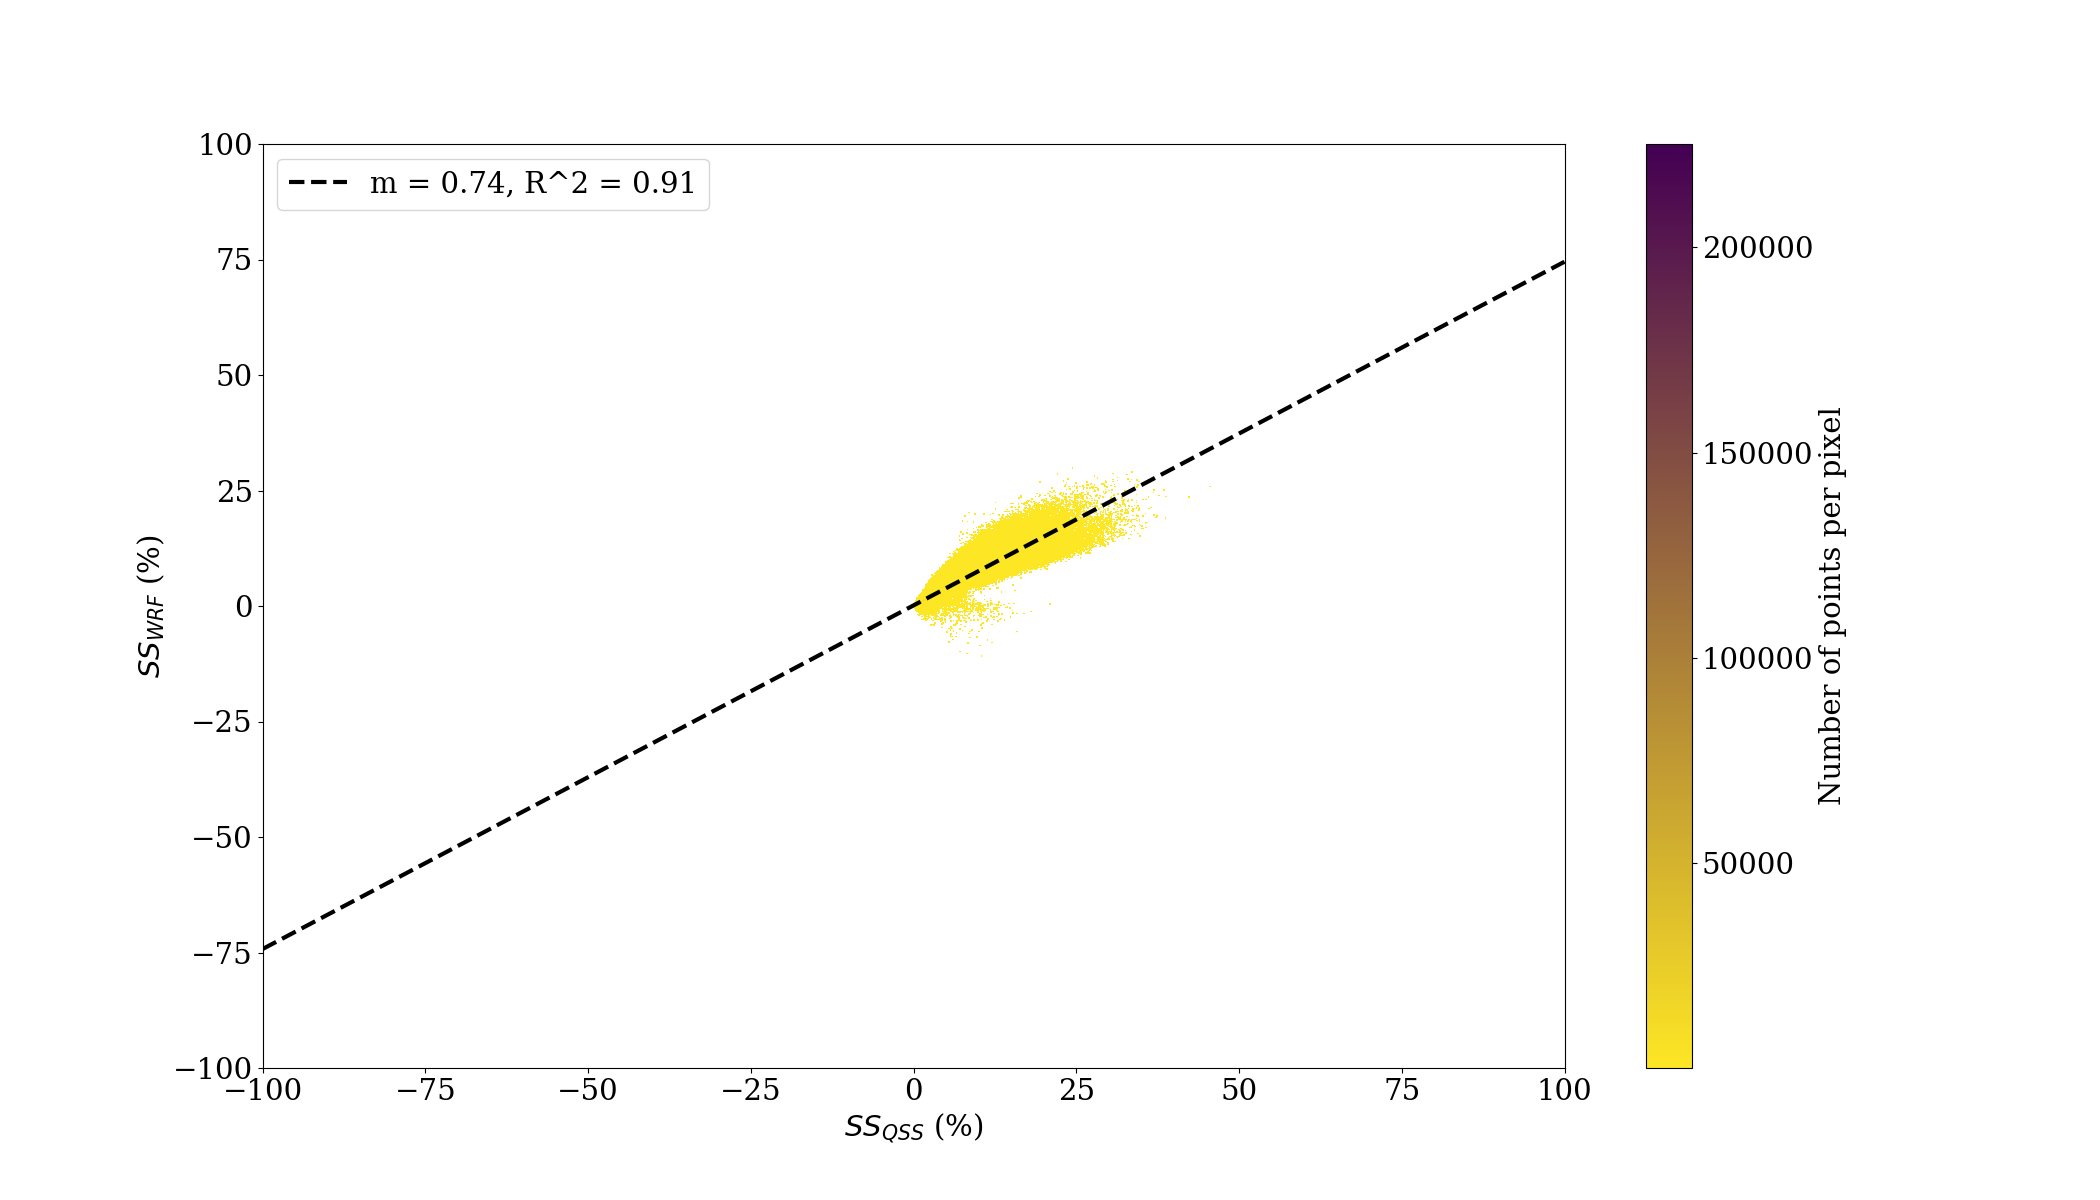
\includegraphics[width=\textwidth]{revmywrf/v12_heatmap_ss_qss_vs_ss_wrf_Unpolluted_figure.png}
		\caption{Unpolluted case.}
		\label{wrfvsqssunpoll}
	\end{subfigure}
	\begin{subfigure}{0.7\textwidth}
		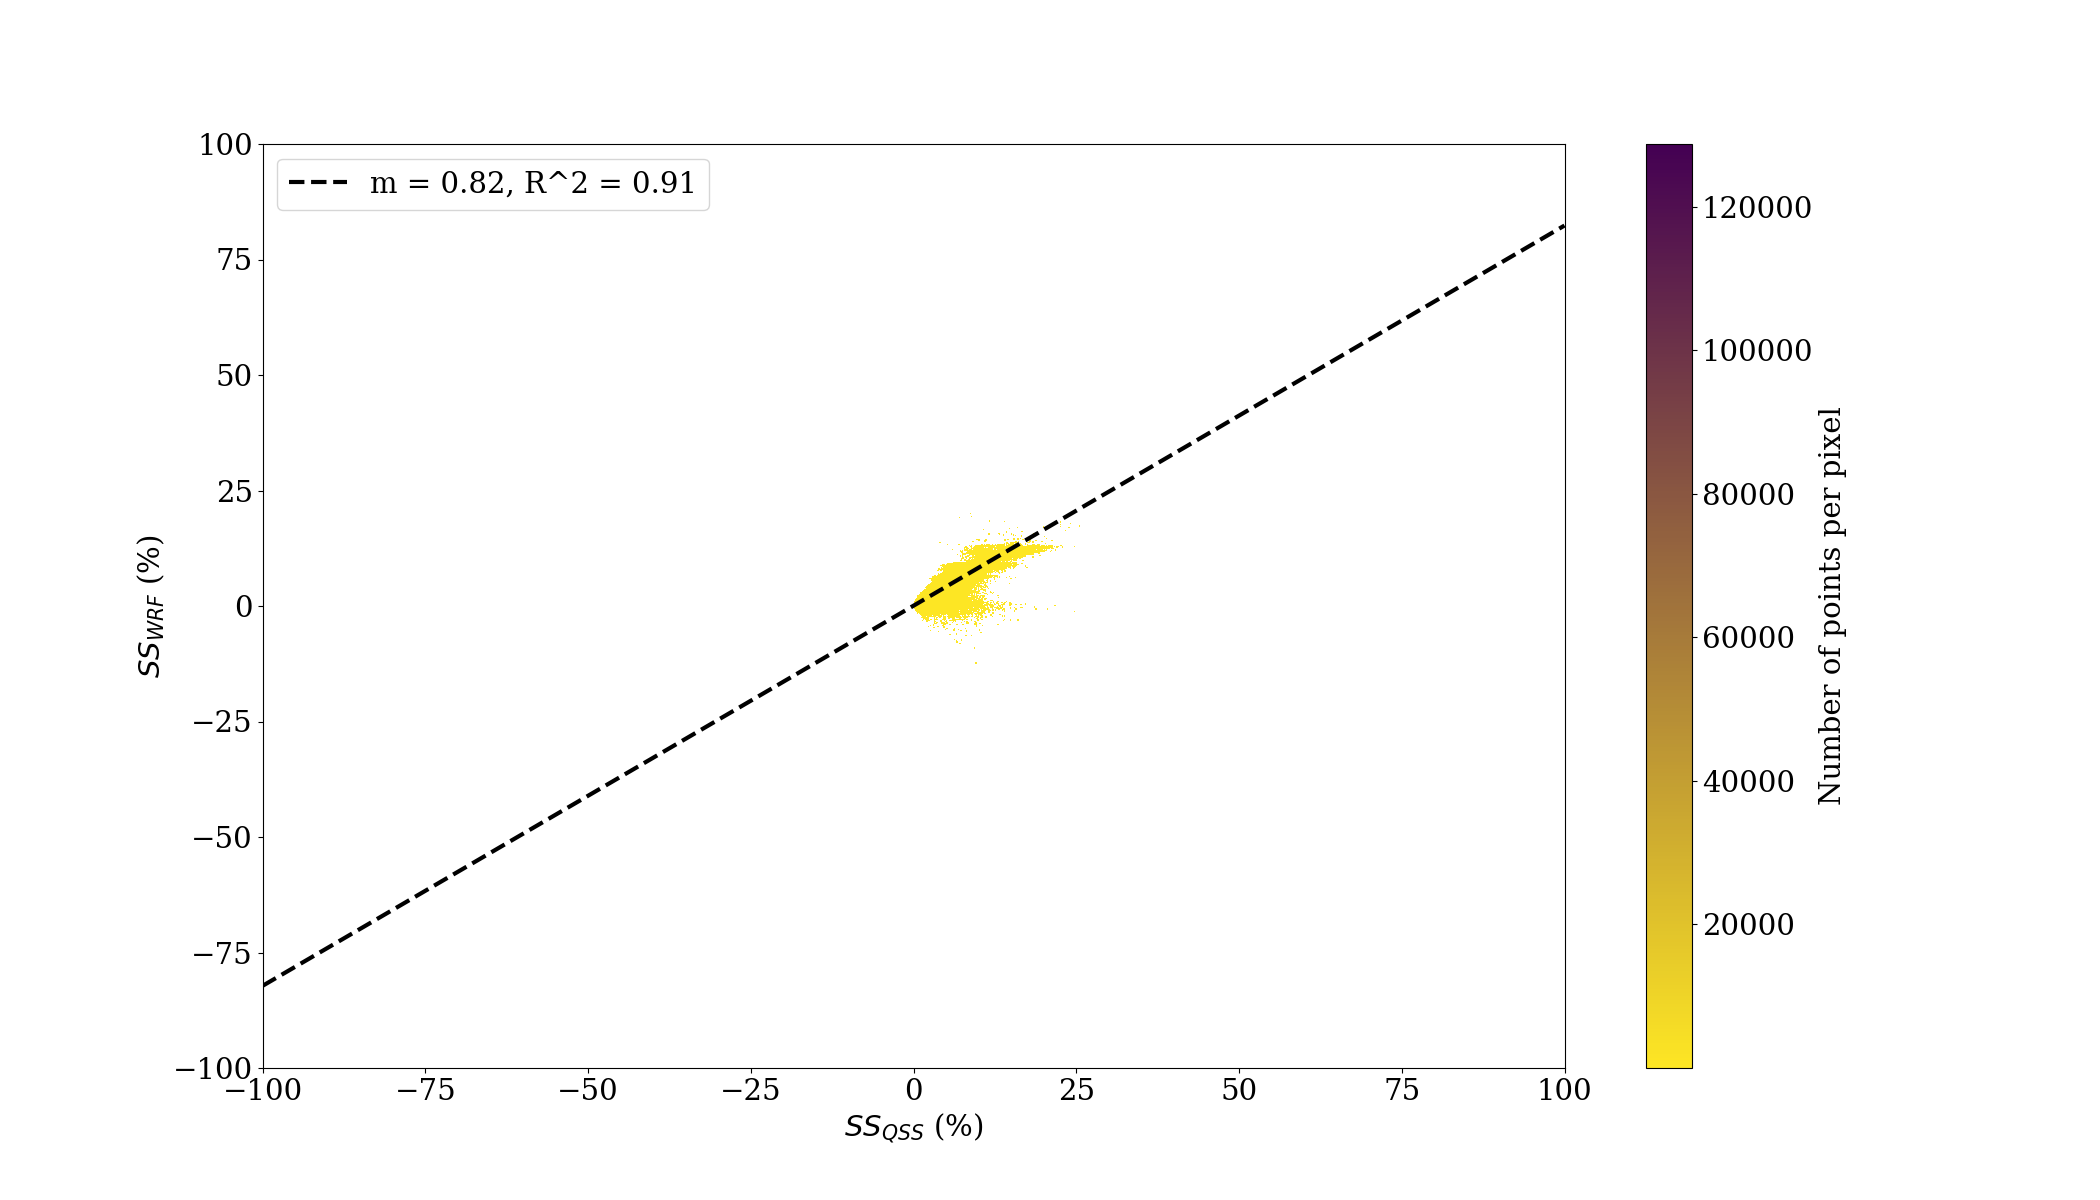
\includegraphics[width=\textwidth]{revmywrf/v12_heatmap_ss_qss_vs_ss_wrf_Polluted_figure.png}
		\caption{Polluted case.}
		\label{wrfvsqsspoll}
	\end{subfigure}
	\caption{Actual ($SS_{WRF}$) vs predicted ($SS_{QSS}$) supersaturation. Histograms show the density of points along each axis.}
	\label{wrfvsqss}
\end{figure}

In Fan 2018, they claim that the so-called warm phase invigoration mechanism (WPIM) is driven by the presence of ultra-fine aerosol particles with sub-50nm diameters (UAP50) on the order of ~1000/ccm in the boundary layer (BL) where cloud droplets are nucleated. Crucial to this argument is the claim that, without such particles present, the troposphere supports very high supersaturations, as observed in simulations (O(10\%)). We seek to determine whether such high values actually occur in nature.

First we look at data from the ACRIDICON-CHUVA mission (part of the HALO campaign) in the Amazon forest in Brazil. Aerosol concentrations in the BL (ie from ground-based measurements) both upwind and downwind of anthropogenic pollution sources on select flight dates are shown in Figures \ref{attoasd} and \ref{goaasd}, respectively.

\clearpage
\newpage

\begin{figure}[ht]
    \centering
    \includegraphics[width=9cm]{atto/atto_psd_figure.png}
    \caption{[DON'T HAVE DATA YET] Aerosol particle size distribution for a representative date; ground-based measurement coinciding with ACRIDICON-CHUVA flight dates, compared to initial distribution in boundary layer for WRF simulation. From ATTO site, upwind of Manaus metropolitan area.}
    \label{attoasd}
\end{figure}
\begin{figure}[ht]
    \centering
    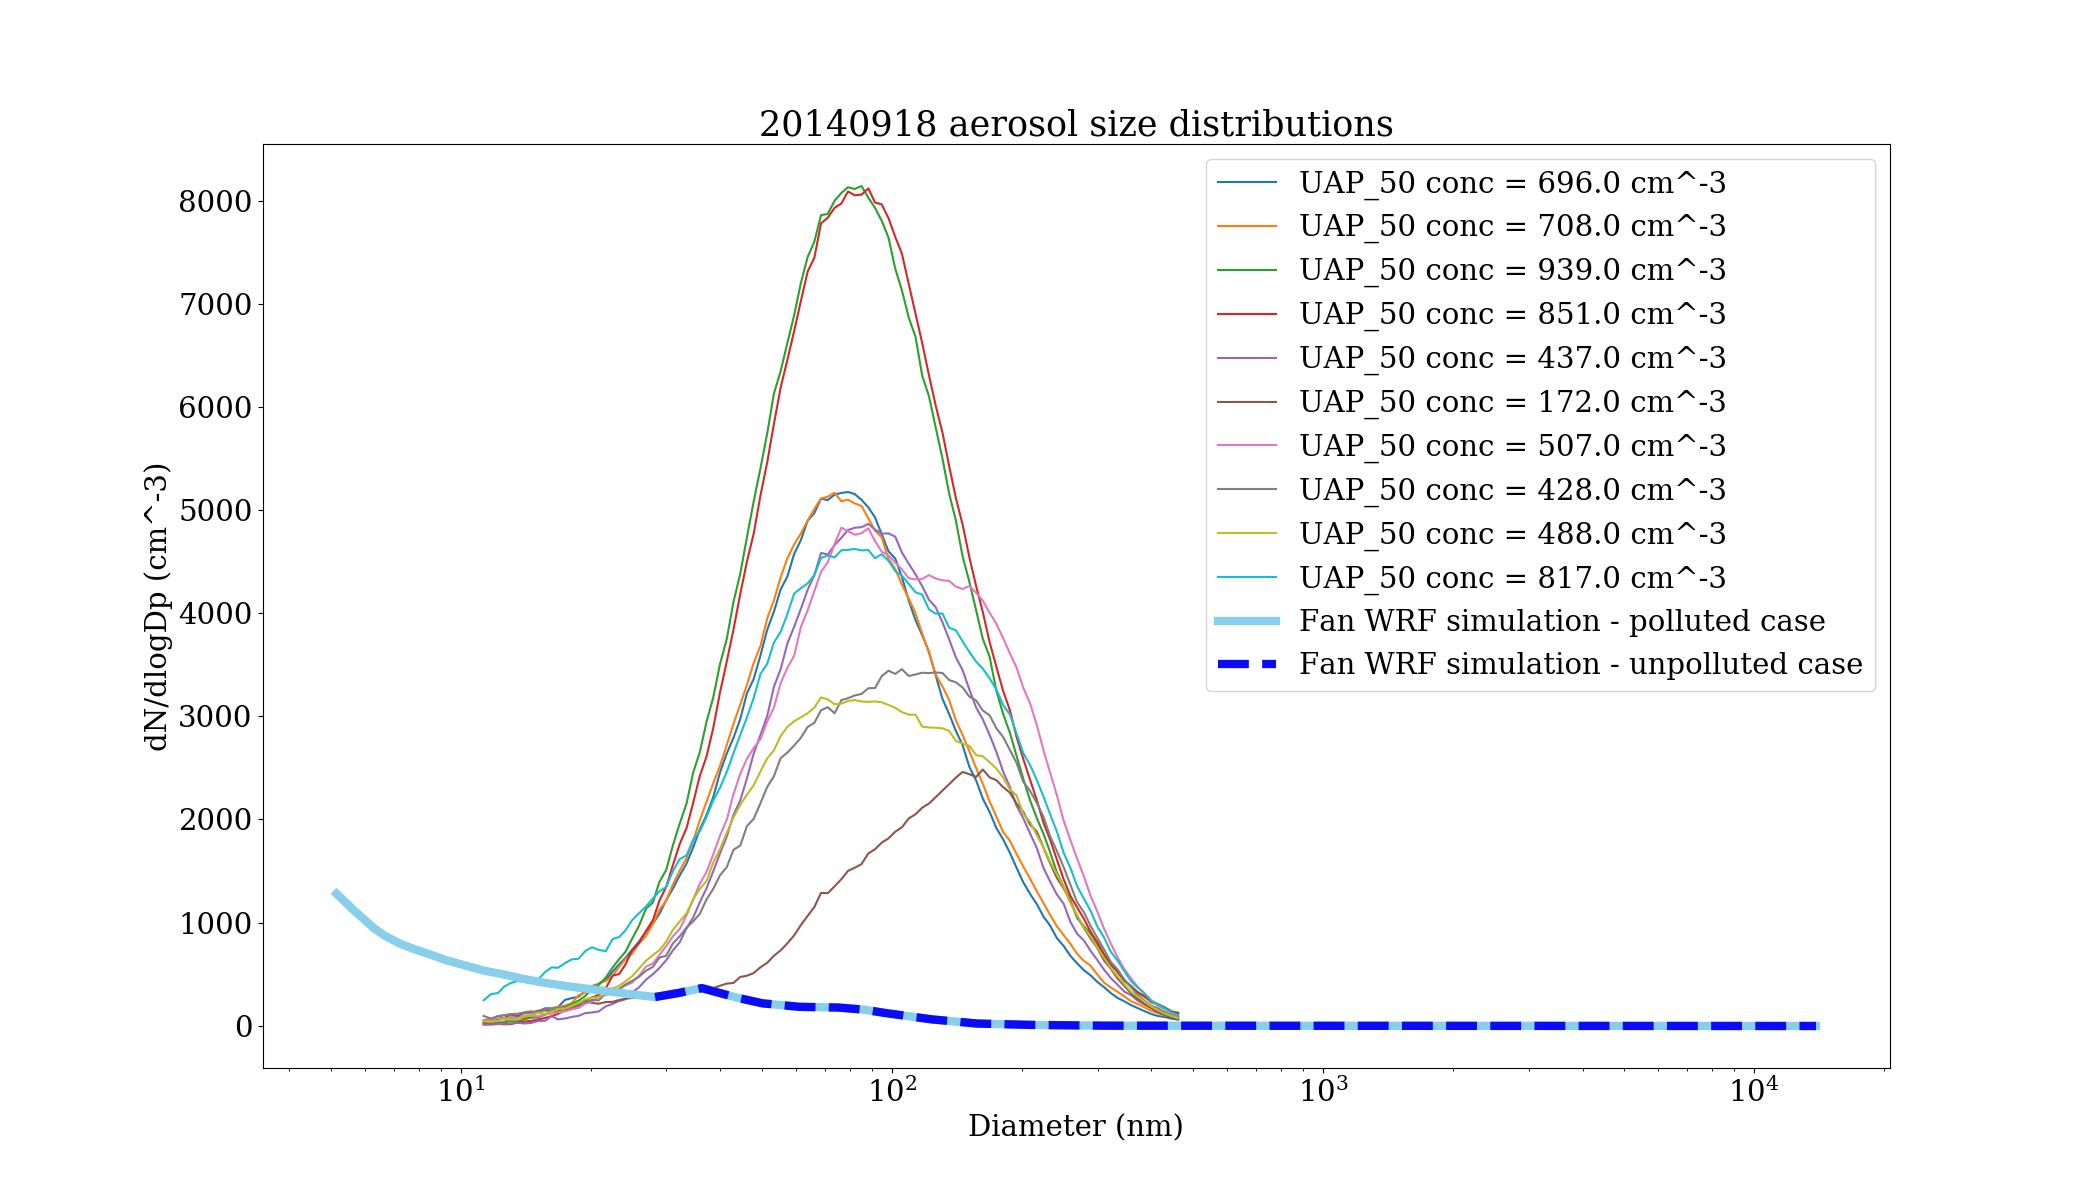
\includegraphics[width=9cm]{goama/v5_aero_size_distb_20140918_figure.png}
    \caption{Aerosol particle size distribution for a representative date; ground-based measurement coinciding with ACRIDICON-CHUVA flight dates, compared to initial distribution in boundary layer for WRF simulation. From GoAmazon site, downwind of Manaus metropolitan area.}
    \label{goaasd}
\end{figure}

Even though UAP50 levels in the BL approach the lower bound of what Fan et al used in their simulations (??? pending ATTO measurements from Mina Pohlker), we do not find any supersaturation values in the troposphere exceeding 1\% using the criteria above (Figure \ref{haloqsshist}).

\clearpage
\newpage

\begin{figure}[ht]
    \centering
    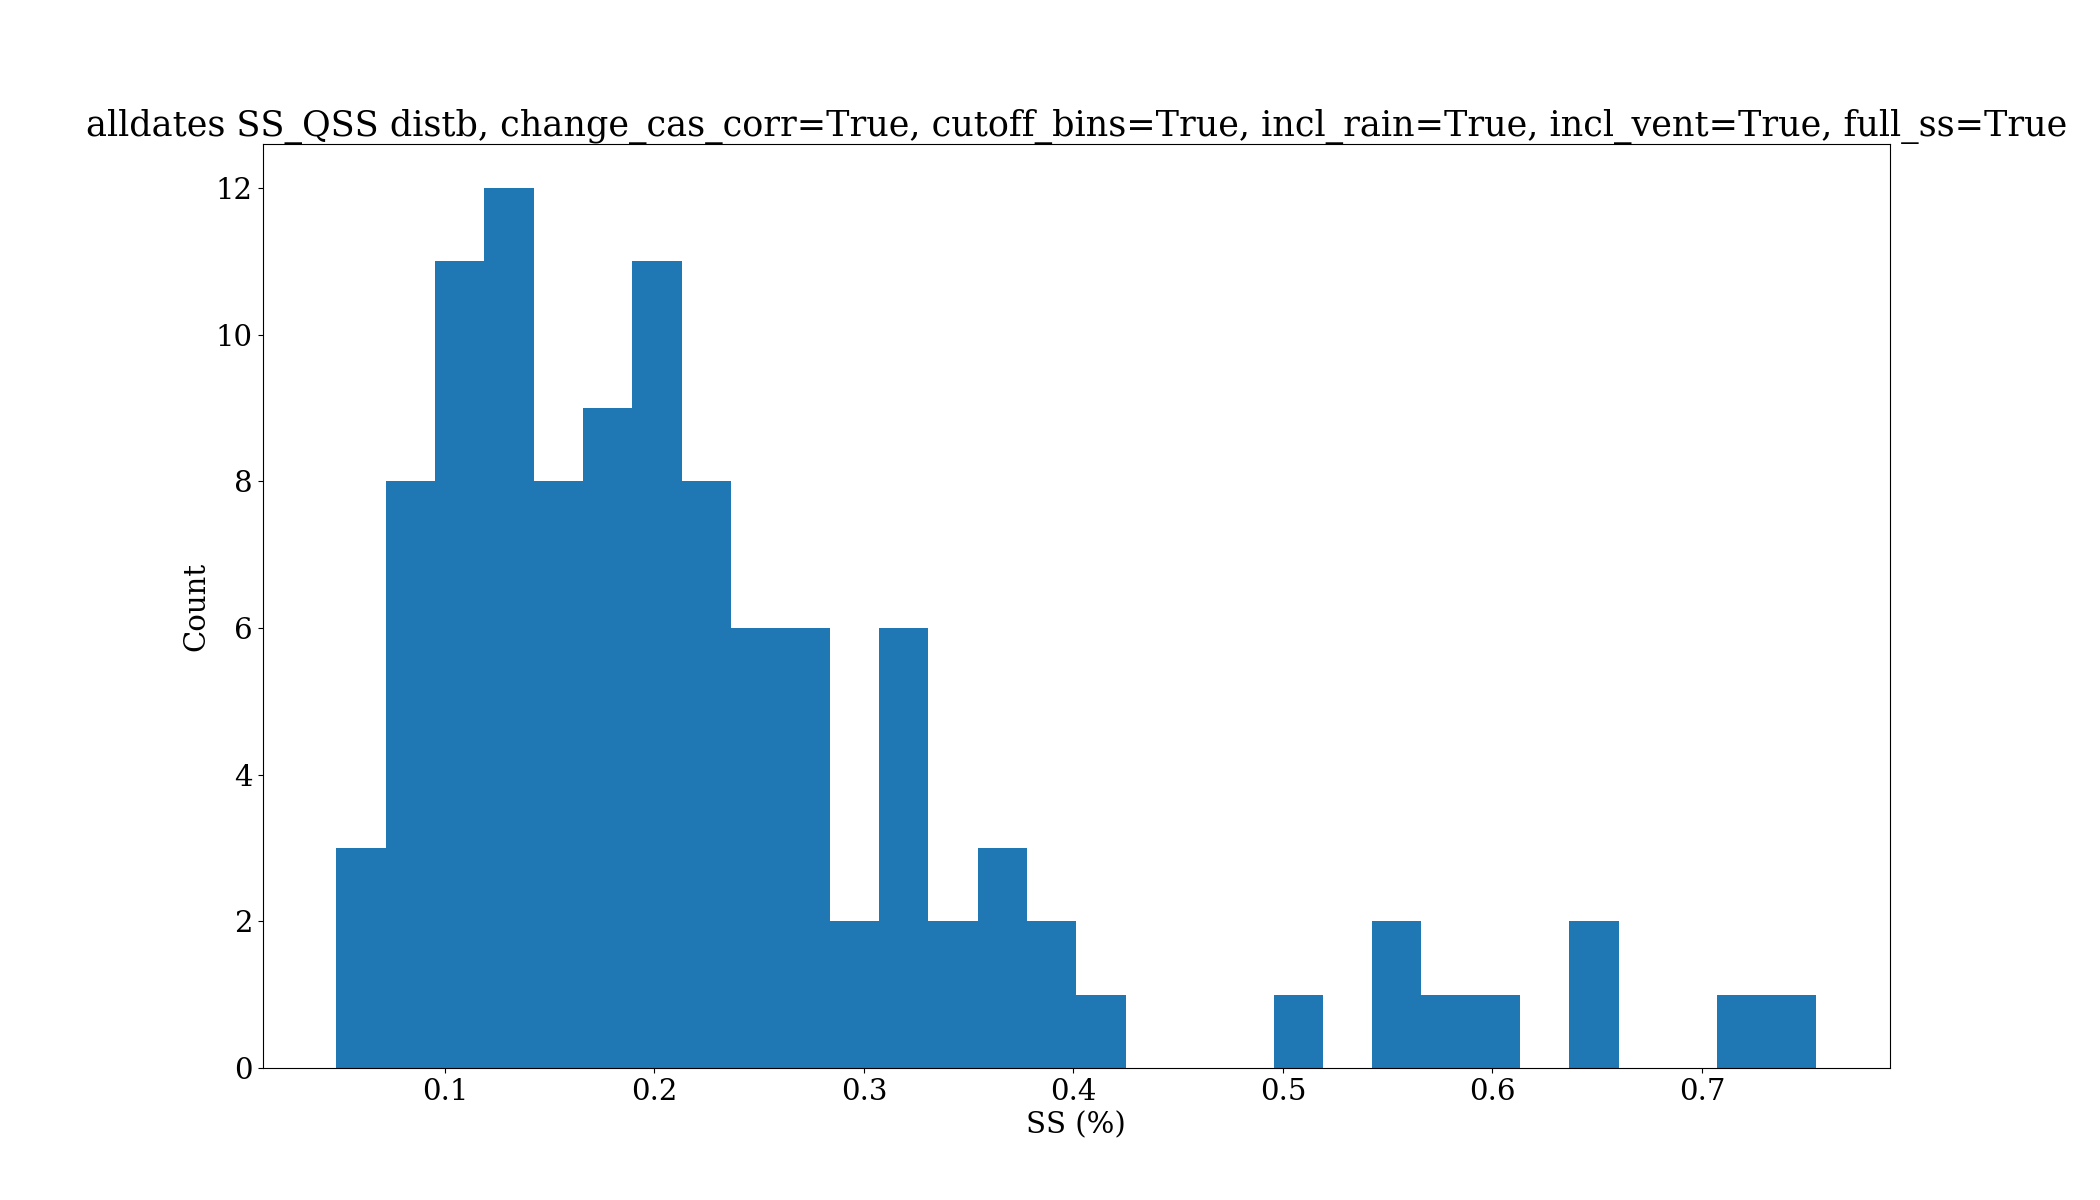
\includegraphics[width=9cm]{revhalo/v24_ss_qss_hist_cas_alldates_figure.png}
    \caption{Predicted ($SS_{QSS}$) supersaturation distribution from HALO field campaign (all flight dates). Using filtering criteria outlined in the text.}
    \label{haloqsshist}
\end{figure}

Next we look at data from the CAIPEEX experiment in India. No ground-based aerosol concentration measurements are available (and measurements in the troposphere from instruments on the plane are sketchy...). Supersaturation distribution using the same criteria is shown (for all flight dates combined) in Figure \ref{caipeexqsshist}. We see a relatively small number of supersaturation values exceeding 1\%.

\begin{figure}[ht]
    \centering
    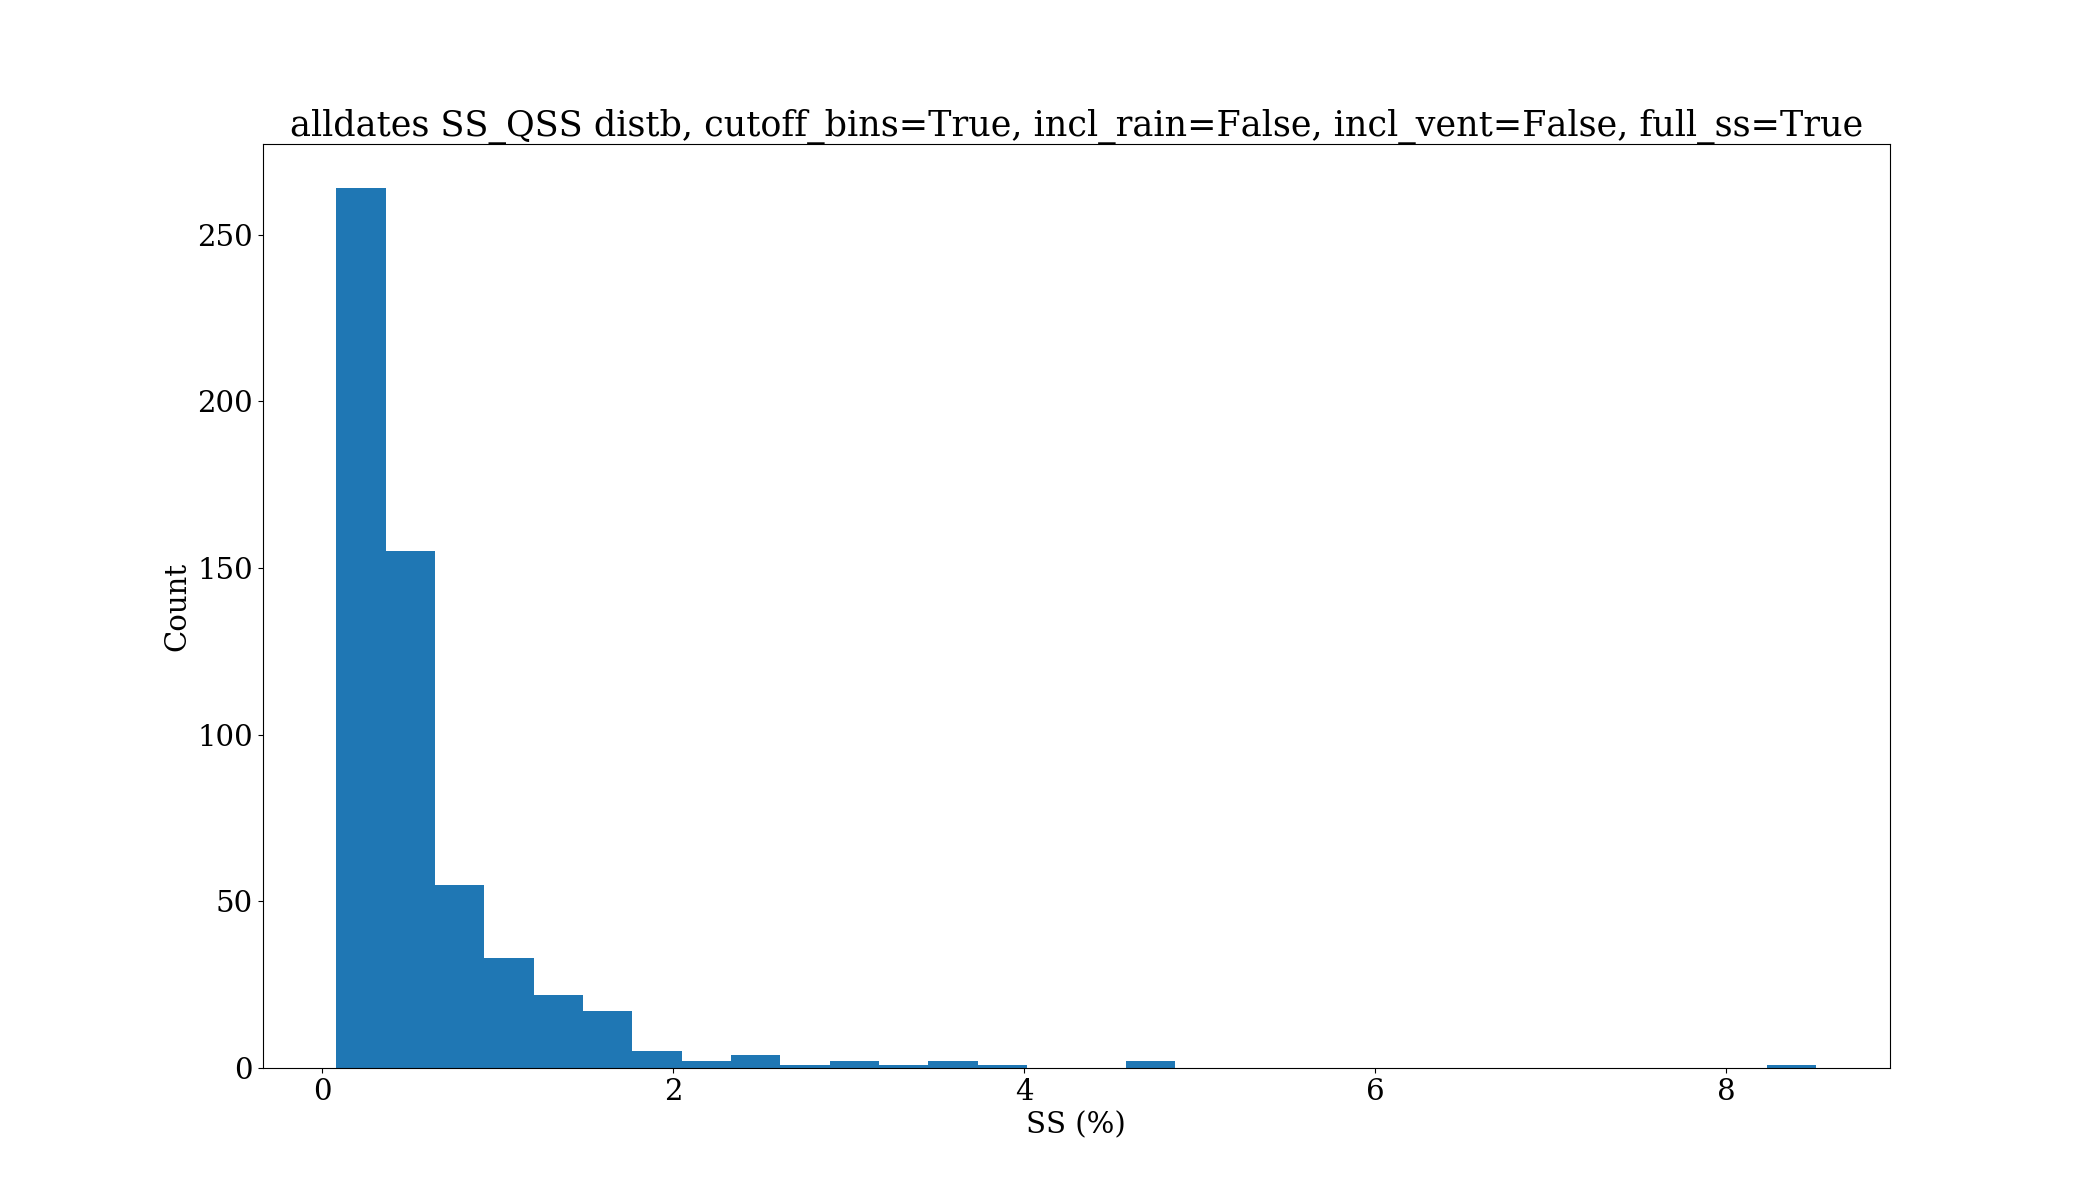
\includegraphics[width=9cm]{revcaipeex/v10_ss_qss_hist_alldates_figure.png}
    \caption{Predicted ($SS_{QSS}$) supersaturation distribution from CAIPEEX field campaign (all flight dates). Using filtering criteria outlined in the text, but not including rain drops or ventilation corrections due to lack of data.}
    \label{caipeexqsshist}
\end{figure}

Conclusion: We do not believe the simulations described in Fan 2018 provide compelling evidence for the legitimacy of the WPIM given that they report supersaturation values far higher than those observed in nature.

One possible counterargument is that the flight campaigns simply didn't fly through strong enough updrafts. However the vertical velocity distributions from the campaigns are quite similar to that from the simulations [can back this up with statistical analysis]. See Figure \ref{combinedwhist}. 

\begin{figure}[ht]
    \centering
    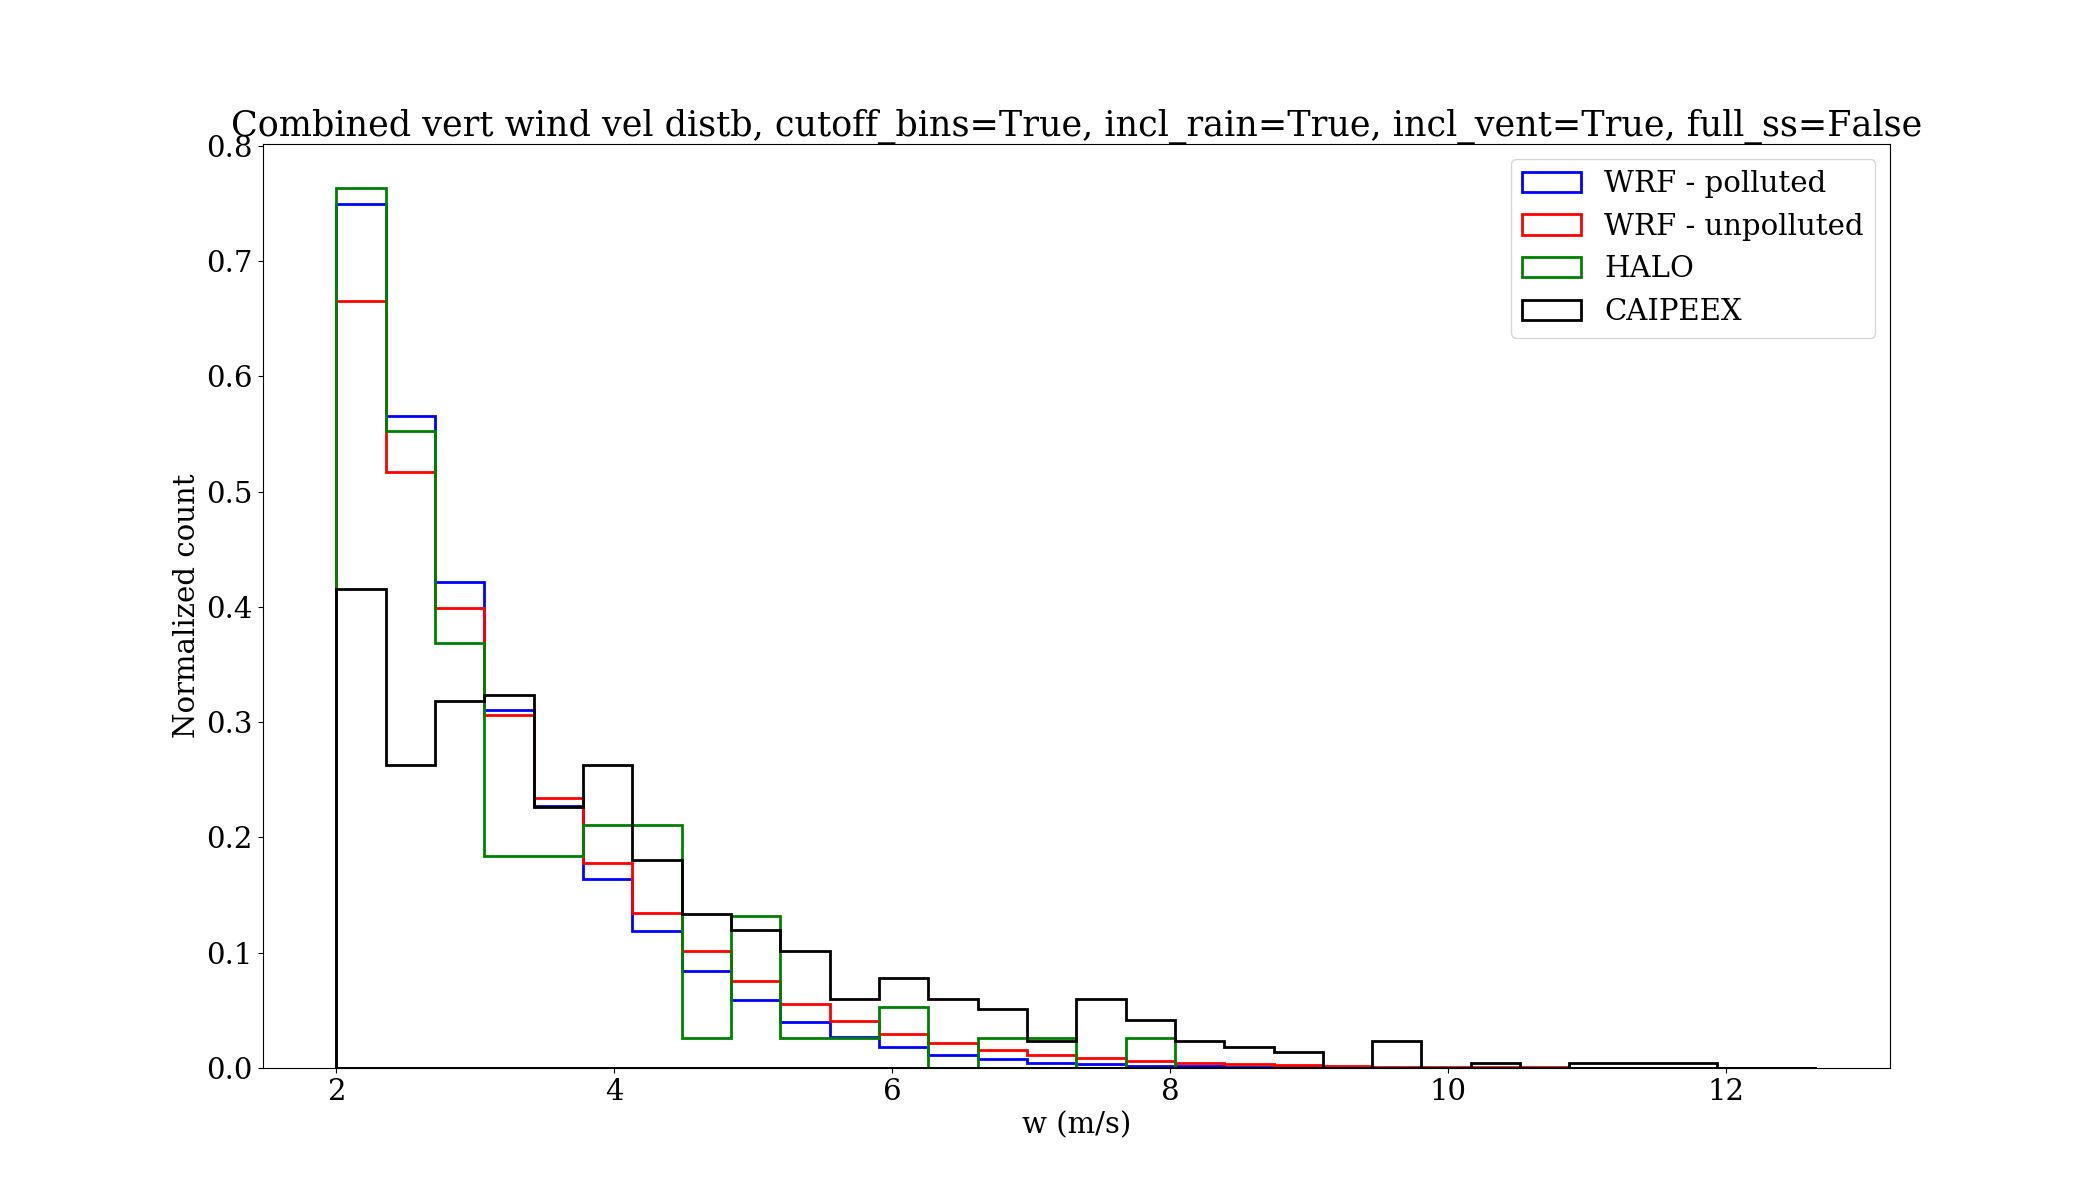
\includegraphics[width=8cm]{revmywrf/v9_combined_w_hist_figure.png}
    \caption{Vertical wind velocity distribution from simulations and field campaigns. Using filtering criteria outlined in the text.}
    \label{halowhist}
\end{figure}

\end{document}
